\documentclass[tikz, border=0pt]{standalone}
\usepackage{pagecolor}

\usepackage{fontspec}
\setsansfont{Inter}[
  BoldFont=Inter Bold,
  Scale=0.92
]

\usepackage{tikz}
\usetikzlibrary{
  shapes.geometric,
  arrows.meta,
  positioning,
  fit,
  calc,
  backgrounds,
  shadows.blur
}

% --- IBM Carbon palette ---
\definecolor{primary}{HTML}{0F62FE}
\definecolor{teal}{HTML}{009D9A}
\definecolor{orange}{HTML}{FF832B}
\definecolor{purple}{HTML}{8A3FFC}
\definecolor{green}{HTML}{198038}
\definecolor{cyan}{HTML}{0072C3}
\definecolor{magenta}{HTML}{D02670}
\definecolor{red}{HTML}{DA1E28}
\definecolor{surface}{HTML}{F4F4F4}
\definecolor{border}{HTML}{A8A8A8}
\definecolor{textprimary}{HTML}{161616}
\definecolor{textsecondary}{HTML}{525252}
\definecolor{arrowcolor}{HTML}{6F6F6F}
\definecolor{bg}{HTML}{151B23}
\definecolor{bglight}{HTML}{161B22}
\pagecolor{bg}

% Layers
\pgfdeclarelayer{background}
\pgfsetlayers{background,main}

% Subtitle command
\newcommand{\nsub}[1]{{\sffamily\tiny\color{textsecondary}#1}}

% --- Styles ---
\tikzset{
  base/.style={
    text=textprimary,
    font=\sffamily\small,
    align=center,
    inner sep=8pt,
  },
  service/.style={
    base,
    draw=#1!60,
    top color=#1!4,
    bottom color=#1!12,
    rounded corners=6pt,
    minimum width=3cm,
    minimum height=1.3cm,
    line width=1.2pt,
    drop shadow={
      shadow xshift=0pt,
      shadow yshift=-2pt,
      opacity=0.15,
      fill=black
    },
  },
  service/.default=primary,
  stor/.style={
    base,
    cylinder,
    shape border rotate=90,
    aspect=0.3,
    draw=#1!60,
    top color=#1!4,
    bottom color=#1!14,
    minimum width=2.4cm,
    minimum height=1.6cm,
    line width=1.2pt,
    drop shadow={
      shadow xshift=0pt,
      shadow yshift=-2pt,
      opacity=0.15,
      fill=black
    },
  },
  stor/.default=primary,
  step/.style={
    base,
    draw=#1!60,
    top color=#1!4,
    bottom color=#1!12,
    rounded corners=5pt,
    minimum width=2.6cm,
    minimum height=1.1cm,
    line width=1.2pt,
    drop shadow={
      shadow xshift=0pt,
      shadow yshift=-1.5pt,
      opacity=0.12,
      fill=black
    },
  },
  step/.default=teal,
  llmnode/.style={
    base,
    draw=purple!60,
    top color=purple!4,
    bottom color=purple!12,
    rounded corners=4pt,
    minimum width=2.2cm,
    minimum height=0.9cm,
    line width=1pt,
    drop shadow={
      shadow xshift=0pt,
      shadow yshift=-1.5pt,
      opacity=0.10,
      fill=black
    },
  },
  container/.style={
    rounded corners=10pt,
    fill=none,
    draw=white!20,
    line width=0.6pt,
    inner sep=14pt,
  },
  clabel/.style={
    font=\sffamily\scriptsize\bfseries,
    text=white,
    anchor=north west,
  },
  flow/.style={
    -{Stealth[length=6pt, width=5pt]},
    line width=1.4pt,
    draw=arrowcolor,
  },
  flowlight/.style={
    -{Stealth[length=5pt, width=4pt]},
    line width=1pt,
    draw=arrowcolor!60,
  },
  elabel/.style={
    font=\sffamily\tiny,
    text=white,
    inner sep=2pt,
  },
}

\begin{document}
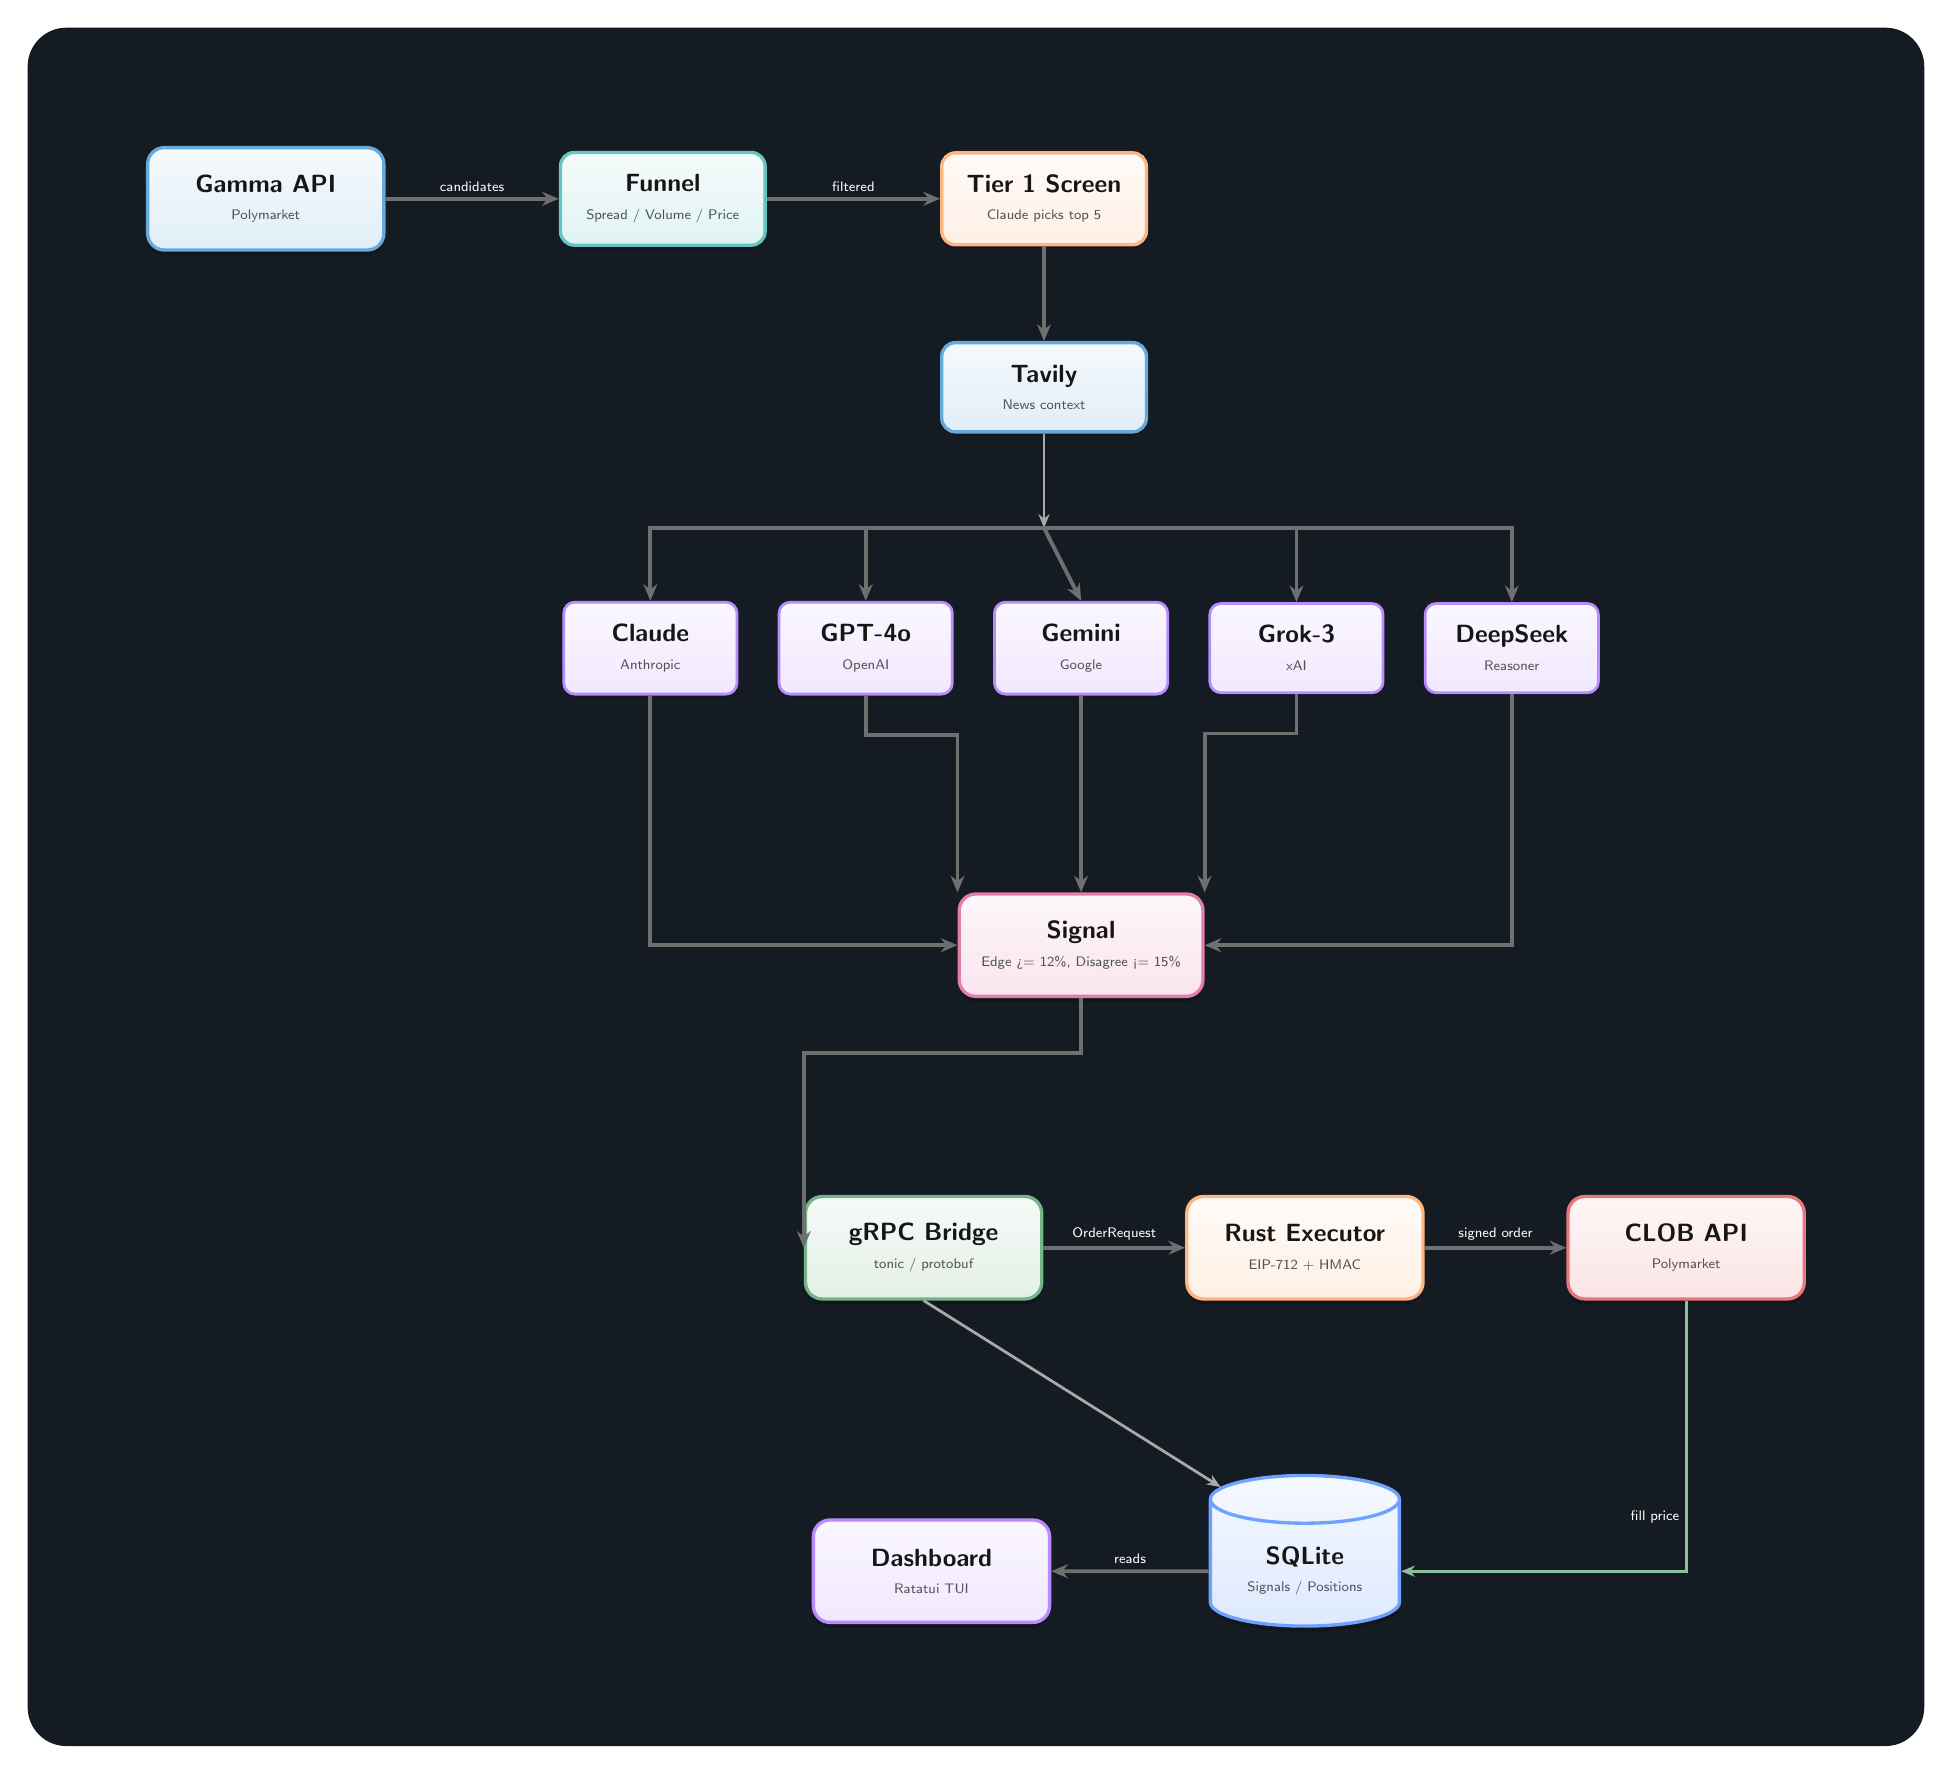
\begin{tikzpicture}

% === ROW 1: Data Sources ===

\node[service=cyan]
  (gamma) {\textbf{Gamma API}\\[-1pt]\nsub{Polymarket}};

\node[step=teal, right=2.2cm of gamma]
  (funnel) {\textbf{Funnel}\\[-1pt]\nsub{Spread / Volume / Price}};

\node[step=orange, right=2.2cm of funnel]
  (screen) {\textbf{Tier 1 Screen}\\[-1pt]\nsub{Claude picks top 5}};

\draw[flow] (gamma) -- node[elabel, above] {candidates} (funnel);
\draw[flow] (funnel) -- node[elabel, above] {filtered} (screen);

% === ROW 2: LLM Consensus ===

\node[llmnode, below=4.5cm of screen, xshift=-5cm]
  (claude) {\textbf{Claude}\\[-1pt]\nsub{Anthropic}};

\node[llmnode, right=0.5cm of claude]
  (gpt) {\textbf{GPT-4o}\\[-1pt]\nsub{OpenAI}};

\node[llmnode, right=0.5cm of gpt]
  (gemini) {\textbf{Gemini}\\[-1pt]\nsub{Google}};

\node[llmnode, right=0.5cm of gemini]
  (grok) {\textbf{Grok-3}\\[-1pt]\nsub{xAI}};

\node[llmnode, right=0.5cm of grok]
  (deep) {\textbf{DeepSeek}\\[-1pt]\nsub{Reasoner}};

% News context
\node[step=cyan, below=1.2cm of screen]
  (tavily) {\textbf{Tavily}\\[-1pt]\nsub{News context}};

% Screen fan-out to LLMs
\coordinate (llmfan) at ($(tavily.south) + (0,-1.2)$);
\draw[flow] (screen.south) -- (tavily.north);
\draw[flowlight] (tavily.south) -- (llmfan);
\draw[flow] (llmfan) -| (claude.north);
\draw[flow] (llmfan) -| (gpt.north);
\draw[flow] (llmfan) -- (gemini.north);
\draw[flow] (llmfan) -| (grok.north);
\draw[flow] (llmfan) -| (deep.north);

% === ROW 3: Signal Generation ===

\node[service=magenta, below=2.5cm of gemini]
  (signal) {\textbf{Signal}\\[-1pt]\nsub{Edge >= 12\%, Disagree <= 15\%}};

% LLMs to signal
\draw[flow] (claude.south) |- (signal.west);
\draw[flow] (gpt.south) -- ++(0,-0.5) -| (signal.north west);
\draw[flow] (gemini.south) -- (signal.north);
\draw[flow] (grok.south) -- ++(0,-0.5) -| (signal.north east);
\draw[flow] (deep.south) |- (signal.east);

% === ROW 4: Execution ===

\node[service=green, below=2.5cm of signal, xshift=-2cm]
  (grpc) {\textbf{gRPC Bridge}\\[-1pt]\nsub{tonic / protobuf}};

\node[service=orange, right=1.8cm of grpc]
  (executor) {\textbf{Rust Executor}\\[-1pt]\nsub{EIP-712 + HMAC}};

\node[service=red, right=1.8cm of executor]
  (clob) {\textbf{CLOB API}\\[-1pt]\nsub{Polymarket}};

\draw[flow] (signal.south) -- ++(0,-0.7) -| (grpc.west);
\draw[flow] (grpc) -- node[elabel, above] {OrderRequest} (executor);
\draw[flow] (executor) -- node[elabel, above] {signed order} (clob);

% === Side: SQLite + Dashboard ===

\node[stor=primary, below=2.2cm of executor]
  (db) {\textbf{SQLite}\\[-1pt]\nsub{Signals / Positions}};

\node[service=purple, left=2cm of db]
  (dash) {\textbf{Dashboard}\\[-1pt]\nsub{Ratatui TUI}};

% Signal to DB
\draw[flowlight] (grpc.south) -- (db.north west);

% DB to dashboard
\draw[flow] (db) -- node[elabel, above] {reads} (dash);

% Executor response back
\draw[flowlight, draw=green!50] (clob.south) |- node[elabel, left, pos=0.4] {fill price} (db.east);

% === Container: Python Strategy ===
\begin{pgfonlayer}{background}
  \node[container, fit=(gamma)(funnel)(screen)(tavily)(claude)(gpt)(gemini)(grok)(deep)(signal),
    label={[clabel]north west:PYTHON STRATEGY LAYER}] {};
\end{pgfonlayer}

% === Container: Rust Execution ===
\begin{pgfonlayer}{background}
  \node[container, fit=(grpc)(executor)(clob),
    label={[clabel]north west:RUST EXECUTION LAYER}] {};
\end{pgfonlayer}

% === Container: Persistence ===
\begin{pgfonlayer}{background}
  \node[container, fit=(db)(dash),
    label={[clabel]north west:PERSISTENCE + MONITORING}] {};
\end{pgfonlayer}

% === Full diagram background ===
\begin{pgfonlayer}{background}
  \fill[bg, rounded corners=14pt]
    ($(current bounding box.south west) + (-1,-1)$)
    rectangle
    ($(current bounding box.north east) + (1,1)$);
\end{pgfonlayer}

\end{tikzpicture}
\end{document}
